\documentclass[11pt]{article}
\usepackage{icmlko}
\begin{document}

\title{공유 열은 도메인을 겹쳐 놓아야 한다 --- 노트 368의 규칙을 뒤집는다}
\author{월드모델 실험실}
\date{노트 369 · 2026년 8월 1일}
\maketitle

\begin{abstract}
노트 368이 규약을 하나 적었다: \emph{공유 열의 눈금은 그 열을 쓰는
도메인 전체에서 한 번 정한다.} 근거는 만화만 새 눈금으로 바꿨을 때 판이
$-0.0029$(1/12) 내려가고 열을 같이 쓰는 세계애니가 제일 크게 다친
것($-0.0063$, 0/12)이었다. \textbf{그 규약대로 해 봤다} --- 세계애니
2,948건의 외부 링크를 마저 받아 두 도메인을 \emph{합친} 분포의 백분위로
매겼다. \textbf{안 낫다}: 판 $-0.0002$(SD 0.0041, 5/12)로 무승부이고
\textbf{팝업이 $-0.0345$(1/12)} 다 --- 노트 367 규약으로 미결정 $\to$
배포 $\to$ 채택 안 함.

그리고 옛 채움을 역산하다가 답이 나왔다. \textbf{옛 채움은 \emph{제
도메인} 백분위였다} --- raw $=$ 외부 링크 수 $+$ 예고편, 값 $=$ 그 도메인
안에서의 백분위. 평균 오차가 만화 0.0176 · 세계애니 0.0105 이고
raw$=$0 에서 정확히 맞는다. \textbf{잃어버린 스크립트가 완전히
복원됐다}(노트 108의 주석 한 줄에서 출발해서).

\textbf{그래서 규칙이 뒤집힌다.} 공유 열은 \emph{도메인 안의 순서}를
나르고, 도메인 사이 차이는 \textbf{원핫 열이 이미 나른다}. 합쳐서 매기면
그 열 안에서 두 도메인이 갈라지는데(예고편이 만화 26\% 대 세계애니 74\%
라 만화가 통째로 내려간다) 그것은 원핫이 하는 말을 한 번 더 하면서
도메인 안의 해상도를 깎는 일이다. \textbf{공유 열은 도메인마다 따로
정규화해 겹쳐 놓는 것이 맞다.}
\end{abstract}

\section{규약대로 해 봤다}

\begin{center}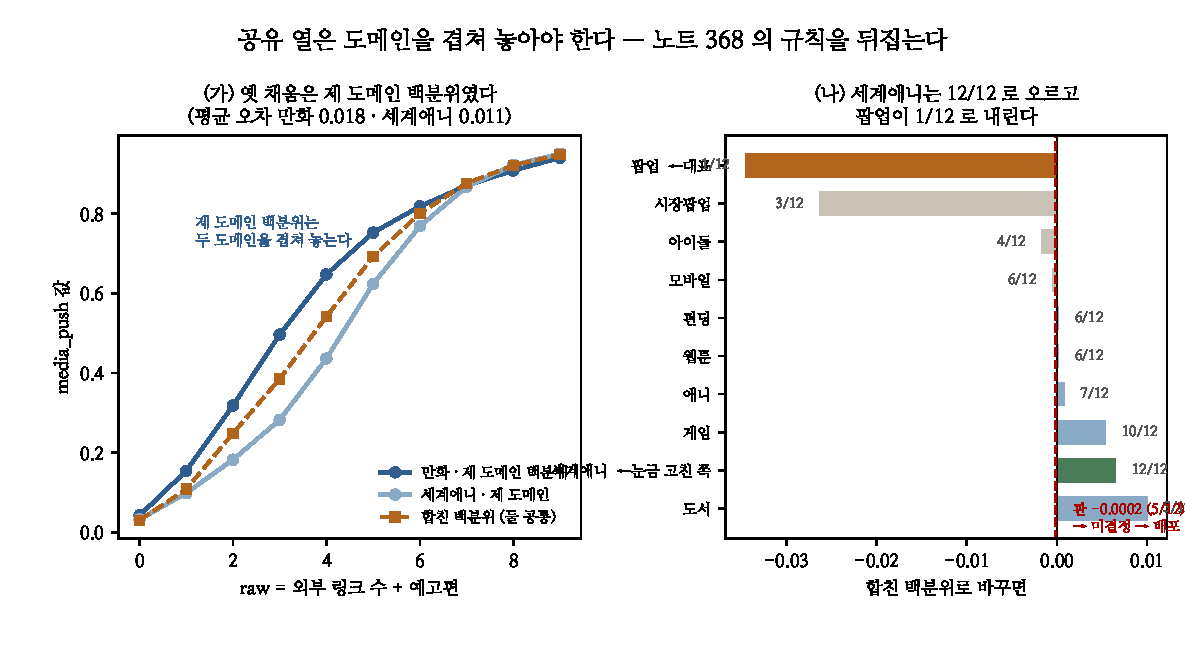
\includegraphics[width=\linewidth]{figs/overlay.pdf}\end{center}

\begin{center}
\begin{tabular}{lrrr}
\hline
합친 백분위로 바꾸면 & 차 & SD & 부호 \\
\hline
\textbf{판} & $-0.0002$ & 0.0041 & 5/12 \\
\textbf{세계애니} & $\mathbf{+0.0065}$ & 0.0048 & \textbf{12/12} \\
게임 & $+0.0054$ & 0.0064 & 10/12 \\
도서 & $+0.0100$ & 0.0291 & 5/12 \\
시장팝업 & $-0.0263$ & 0.0376 & 3/12 \\
\textbf{팝업}(대표) & $\mathbf{-0.0345}$ & 0.0168 & \textbf{1/12} \\
\hline
\end{tabular}
\end{center}

노트 367 규약: $|-0.0002| < 2{\times}$SD$(0.0081)$ 이고 부호 5/12 가
$[4,8]$ 안 $\Rightarrow$ 미결정 $\Rightarrow$ 배포가 정한다 $\Rightarrow$
팝업 1/12 $\Rightarrow$ \textbf{안 넣는다.}

\textbf{다만 세계애니는 12/12로 오른다.} 눈금을 고쳐 준 바로 그 도메인이
일관되게 좋아진다 --- 노트 368의 진단(``세계애니가 만화의 눈금 때문에
다쳤다'')은 맞았다. \textbf{틀린 것은 처방이다.}

\section{옛 채움을 복원했다}

역산했다. 옛 값과 ``외부 링크 수 $+$ 예고편''의 순위 상관이 만화
$+0.9905$ · 세계애니 $+0.9921$ 이다(링크만 쓰면 $+0.9523$ · $+0.9601$ 로
떨어진다 --- \textbf{예고편이 들어간다}). 그리고 눈금은

\begin{center}
\begin{tabular}{rrrrr}
\hline
raw & 만화 제도메인CDF & 만화 옛 값 & 세계애니 제도메인CDF & 세계애니 옛 값 \\
\hline
0 & 0.042 & \textbf{0.042} & 0.032 & \textbf{0.032} \\
1 & 0.154 & 0.151 & 0.098 & 0.088 \\
2 & 0.318 & 0.308 & 0.182 & 0.150 \\
3 & 0.496 & 0.472 & 0.282 & 0.308 \\
5 & 0.752 & 0.714 & 0.623 & 0.629 \\
8 & 0.908 & 0.918 & 0.922 & 0.923 \\
\hline
\multicolumn{5}{c}{평균 오차 --- 만화 0.0176 · 세계애니 0.0105} \\
\hline
\end{tabular}
\end{center}

\textbf{제 도메인 백분위다.} 노트 365가 ``만든 스크립트가 없어 눈금
역산은 추측이 된다''고 접었던 것이 완전히 복원됐다 ---
\texttt{ingest/media\_push.py} 로 다시 쓰면 옛 값과 순위 상관 $+0.9905$ ·
$+0.9932$ 가 나온다.

\textbf{개념을 주석에 남기는 것이 두 번째로 값을 했다}(노트 368에 이어).
노트 108의 ``공식 외부 채널 수와 예고편 유무'' 한 줄이 없었다면 이
복원은 못 했다.

\section{그래서 규칙이 뒤집힌다}

\begin{quote}
\textbf{노트 368}: 공유 열의 눈금은 그 열을 쓰는 도메인 전체에서 한 번
정한다. \\
\textbf{노트 369(정정)}: 공유 열은 \emph{도메인마다} 정규화해
\textbf{겹쳐 놓는다.}
\end{quote}

\textbf{까닭.} F18은 도메인마다 원핫 열을 하나씩 붙인다 --- ``이 행이 어느
도메인인가''는 이미 그 열이 말한다. 공유 열이 할 일은 \emph{그 도메인
안에서 이 행이 몇 등인가}이고, 도메인마다 $[0,1]$ 로 펴 놓으면 그 정보가
최대가 된다. 합쳐서 매기면 두 도메인이 열 안에서 서로 다른 구간에 놓여
(만화 중앙 0.363 대 세계애니 0.516) 원핫이 하는 말을 되풀이하면서
각 도메인의 순위 해상도를 깎는다.

\textbf{노트 368이 왜 틀렸나.} 그 노트가 잰 것은 ``만화만 눈금을 바꾸면
나쁘다''였고, 거기서 ``그러니 합쳐서 매겨야 한다''로 갔다. 실제 원인은
\emph{합쳐야 해서}가 아니라 그 새 눈금이 만화를 $[0.25,0.75]$ 로
\textbf{눌러서} 도메인 안 해상도를 잃었기 때문이다. \textbf{두 처방이
같은 증상을 설명하는데 하나만 맞았다} --- 이번 창에서 세 번째다
(노트 353 · 360 · 369).

\section{그리고 벽이 없어졌다}

노트 365 · 366 · 368이 만화 258행 앞에 세운 벽은 ``채움을 다시 만들 수
없다''였다. \textbf{이제 만든다} --- 제 도메인 백분위로 2,041행을 채우면
된다. 마지막 게이트를 돌리고 있다(옛 채움 대 재현, 그리고 258행 추가).

\section{남은 것}

\begin{center}
\begin{tabular}{ll}
\hline
갈래 & 지금 아는 것 \\
\hline
\textbf{만화 258행} & 채움 재현 게이트 돌리는 중. 지나면 넣는다 \\
세계애니 눈금 & 합친 백분위가 세계애니를 12/12 로 올린다. \\
 & 그 도메인만 따로 손볼 여지가 있나 \\
팝업 실측 41행 & 노트 360 · 364 · 366 \\
\hline
\end{tabular}
\end{center}

둘째 줄이 새 갈래다 --- 합침이 세계애니에는 좋고 팝업에는 나빴다.
같은 처치가 도메인마다 갈리는 자리는 노트 258이 ``전용 축은 공짜가
아니다''로 처음 적은 것과 같은 집안이다.

\end{document}
